\documentclass[10pt]{article}
\usepackage{enumitem}
\usepackage{parskip}
\usepackage[T1]{fontenc}
\usepackage[utf8]{inputenc}
\usepackage{listings}
\usepackage{hyperref}
\usepackage{tikz}
\usepackage{enumitem}
\usepackage[Q=yes]{examplep}
\usepackage{graphicx}
\usepackage{multicol}

\newcommand{\command}[1]{\texttt{#1}}
\newcommand{\escape}[1]{\PVerb{#1}}

\begin{document}

  % Title page.
  %------------

  \thispagestyle{empty}
  \vspace*{3cm}
  \begin{center}
    \huge{EITN50 -- Advanced Computer Security} \\
    \vspace{0.3cm}
    \LARGE{Anatomy of an Exploit} \\
    \vspace{1cm}
    \large{by: \\ \vspace{0.2cm}
	\textit{adsec03} \\
        Stefan Eng \texttt{<atn08sen@student.lu.se>} \\
        Rasmus Olofzon \texttt{<muh11rol@student.lu.se>}
        } \\
  \end{center}

  % First page
  %-----------

  \newpage

  \section*{Introduction}

  \section{Assignments}

    \subsection{Assignment 1 -- Running the exploit}

      Executing the python file exploit.py without the software started resulted in a
      command prompt displays the following:
      \begin{verbatim}
  [*] Connecting to 192.168.0.1...
      \end{verbatim}
      with nothing else happening.

      Analyzing the exploit script reveals that it tries to connect to and
      exploit an instance of \textit{Easy File Management Web Server v5.3} to trigger a
      remote buffer overflow. If the exploit is successful, it should close the
      management software and bring up an instance of the Windows calculator.

      After starting the web management software and running the exploit again,
      this is what happens.

    \subsection{Assignment 2}
       In the exploit.py file a \texttt{payload} string is constructed. Most of
       the parts it is constructed with are hex values packed in an unsigned
       long little endian fashion (e. g. \escape{pack('<L',0x10022aac)}). A
       relatively low-risk guess is that these hex values are memory addresses
       for different gadgets used in the attack. This is also in part confirmed
       by the comments supplied in the code. Some parts are also \escape{\x90}
       repeated a number of times.  \escape{\x90} in x86 architecture
       corresponds to the NOP operation, which does nothing (stands for no
       operation). Last in the \texttt{payload} is a \texttt{shellcode} string,
       which after consulting
       \escape{https://defuse.ca/online-x86-assembler.htm} seems to be x86
       instructions.

       \newpage

      This is a schematic representation of the stack before the overflow has
      occurred.

      \begin{multicols}{3}
        \input{input/stack_before_0.tex}
        \input{input/stack_before_1.tex}
        \input{input/stack_before_2.tex}
      \end{multicols}

      These are the same relative positions after the overflow has occurred.

      \input{input/stack_after.tex}

      Clarification of which instructions the different gadgets are composed
      of.

      \begin{description}[style=multiline,leftmargin=3.5cm]
        %\item[junk0]{80 \texttt{NOP}}
        \item[call\_edx]{\texttt{JMP 0xffffffda \\
                                 ADD DWORD PTR [EAX],EDX}}
        %\item[junk1]{280 \texttt{NOP}}
        \item[ppr]{\texttt{%
            POP EBX \\
            POP ECX \\
            RETN
        }}
        \item[crafted\_jmp\_esp]{\texttt{%
            JMP ESP
        }}
        \item[test\_bl]{\texttt{%
            ADD BYTE PTR DS:[EAX],AL
        }}
        \item[kungfu]{\texttt{%
            MOV EAX,EBX\\
            POP ESI\\
            POP EBX\\
            RETN\\
            %DEADBEEF \\
            %DEADBEEF \\
            ADD EAX,5BFFC883\\
            RETN\\
            PUSH EAX\\
            RETN
        }}
      \end{description}

    \subsection{Assignment 3}

      After attaching to the software and putting a breakpoint at the address
      \\
      \escape{0x00468702}, the following instructions were run until the
      execution hit the shell-code payload.

      \input{input/command_selection.tex}

      where the marked entries were those deemed most vital for the exploit
      functionality.

      \begin{description}[style=multiline]
        \item[00]{
          The entry point of the exploit since the overflow makes it
          possible to specify the value of \escape{EDX}.
        }
        \item[09-14{
          This sequence enables the stack-pivot to occur. This makes the
          execution to continue
        }
      \end{description}

      \begin{verbatim}
        [Numbered list of exploites picked from the list above]
      \end{verbatim}

      The purpose of each of these instructions is documented below.

      \begin{verbatim}
        [Enumerated / Description environment that explains all
        the highlighted instructions from above]
      \end{verbatim}

      With the other instructions doing the following:

      \begin{verbatim}
        [ Discussion about the other instructions and their purpose ]
      \end{verbatim}

      The filler is there to [...]


      \begin{verbatim}
        [ Discussion about NOP-sleads (+ pictures) ]
      \end{verbatim}


    \subsection{Assignment 4}

Firstly, since the memory addresses specified in exploit.py are constants, this tells us that at least ImageLoad.dll (where the parts of the payload that are not \texttt{shellcode} are injected) does not have ASLR enabled. However, let us look for some answers:

From Microsoft's documentation for ISVs (Independent Software Vendor) (\escape{https://msdn.microsoft.com/en-us/library/bb430720.aspx}) we find that:

\begin{itemize}
	\item "ASLR moves executable images into random locations when a system boots [..]" \\
	\item "By default, Windows Vista and later will randomize system DLLs and EXEs, but  DLLs and EXEs created by ISVs must opt in to support ASLR using the /DYNAMICBASE linker option."
%\end{itemize}
	\item "ASLR also randomizes heap and stack memory:

\begin{itemize}
		\item When an application creates a heap in Windows Vista and later, the heap manager will create that heap at a random location to help reduce the chance that an attempt to exploit a heap-based buffer overrun succeeds. Heap randomization is enabled by default for all applications running on Windows Vista and later.
		\item When a thread starts in a process linked with /DYNAMICBASE, Windows Vista and later moves the thread's stack to a random location to help reduce the chance that a stack-based buffer overrun exploit will succeed"
	\end{itemize}
\end{itemize}

This tells us that if ASLR is enabled, the location for executables is randomised at system boot, the location for application heap is randomised at heap creation and the location for a thread's stack is randomised at process start.
%This means that if ASLR is enabled, heap and stack memory addresses should change between program executions (in our case debugging sessions) and application's location in memory should change after a restart of the virtual machine. Let us try that, but first let us take a theoretical (sort of) approach to this:
From this (\escape{https://stackoverflow.com/questions/39189477/how-do-i-determine-if-an-exe-or-dll-participate-in-aslr-i-e-is-relocatable}) answer to a StackOverflow question we see how we can check if the ISV has opted in to support ASLR, as described above. This is also described in Microsoft's own documentation on file headers:

\begin{itemize}
	\item In the \escape{IMAGE_FILE_HEADER} structure we can see that if the flag \escape{IMAGE_FILE_RELOCS_STRIPPED = 0x0001} is set in the Characteristics field, this means that the file is not relocatable. (\escape{https://msdn.microsoft.com/en-us/library/windows/desktop/ms680313(v=vs.85).aspx})

	\item In the \escape{IMAGE_OPTIONAL_HEADER} structure we can see that the if flag \escape{IMAGE_DLLCHARACTERISTICS_DYNAMIC_BASE = 0x0040} is set in the DLLCharacteristics field, it means that the file can be relocated at load time (relate this to /DYNAMICBASE from above). (\escape{https://msdn.microsoft.com/en-us/library/windows/desktop/ms680339(v=vs.85).aspx})
\end{itemize}

As suggested in the StackOverflow answer mentioned above, we installed PEView and checked the file headers for ImageLoad.dll and fmws.exe. See figures \ref{relocImg}, \ref{dynamicImg}, \ref{reloc-fmws} and \ref{dynamic-fmws} for this.

\begin{figure}
	\caption{\escape{IMAGE_FILE_RELOCS_STRIPPED} is not set \escape{=>} ImageLoad.dll is relocatable.}\vspace{0.2em}
	\label{relocImg}
	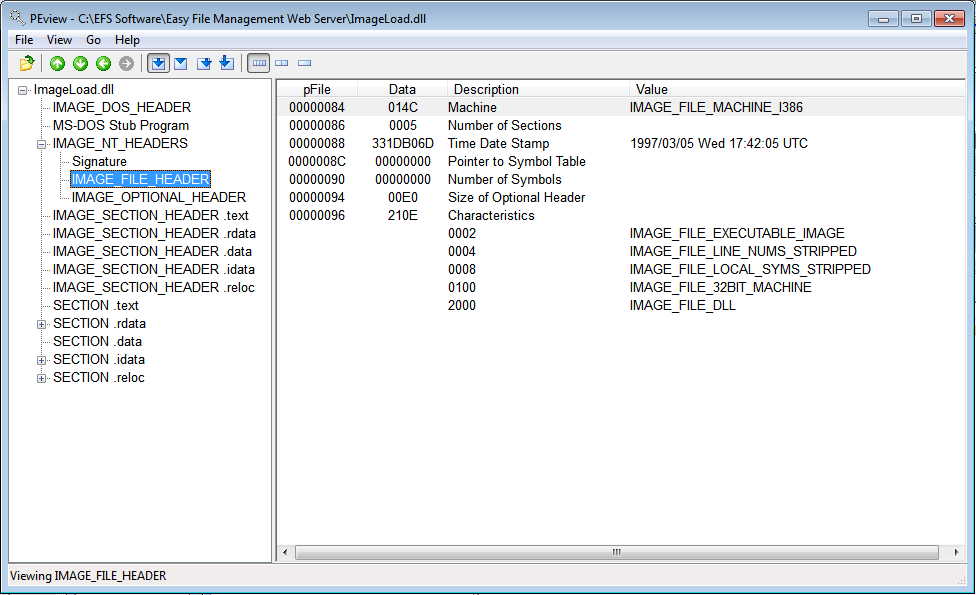
\includegraphics[width=\textwidth]{noRelocImageLoad.png}
\end{figure}

\begin{figure}
	\caption{\escape{IMAGE_DLLCHARACTERISTICS_DYNAMIC_BASE} is not set \escape{=>} ImageLoad.dll is not relocated at load time \escape{=>} ASLR not enabled.}\vspace{0.2em}
	\label{dynamicImg}
	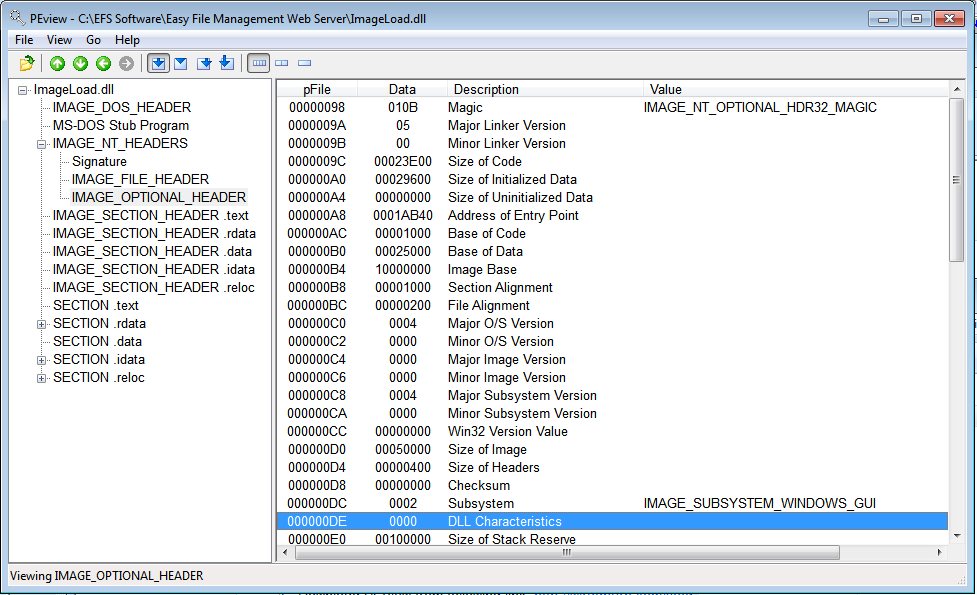
\includegraphics[width=\textwidth]{noASLRforImageLoad.png}
\end{figure}

\begin{figure}
	\caption{\escape{IMAGE_FILE_RELOCS_STRIPPED} is set \escape{=>} fmws.exe is not relocatable.}\vspace{0.2em}
	\label{reloc-fmws}
	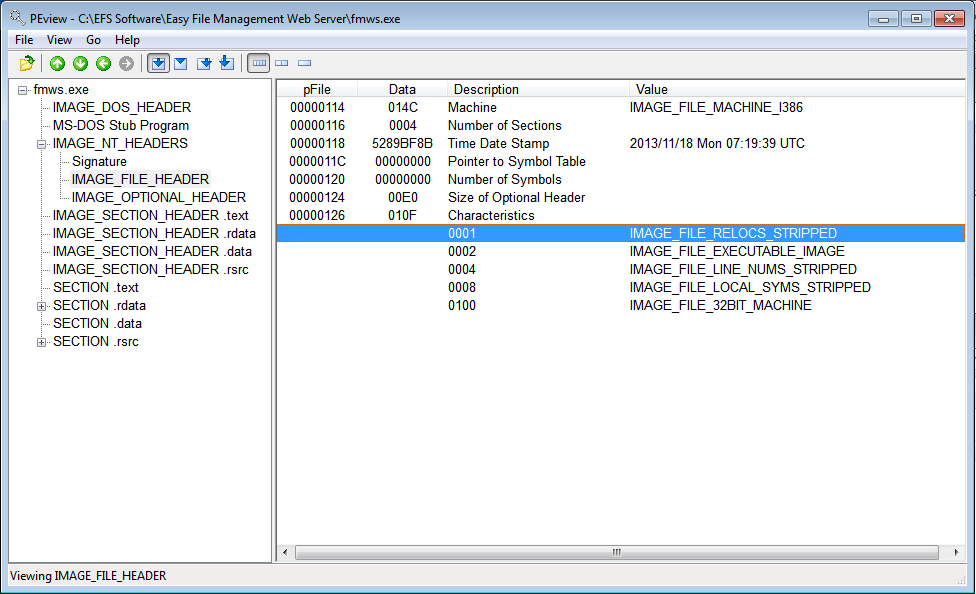
\includegraphics[width=\textwidth]{relocfmws.png}
\end{figure}

\begin{figure}
	\caption{\escape{IMAGE_DLLCHARACTERISTICS_DYNAMIC_BASE} is not set \escape{=>} fmws.exe is not relocated at load time \escape{=>} ASLR not enabled.} \vspace{0.2em}
	\label{dynamic-fmws}
	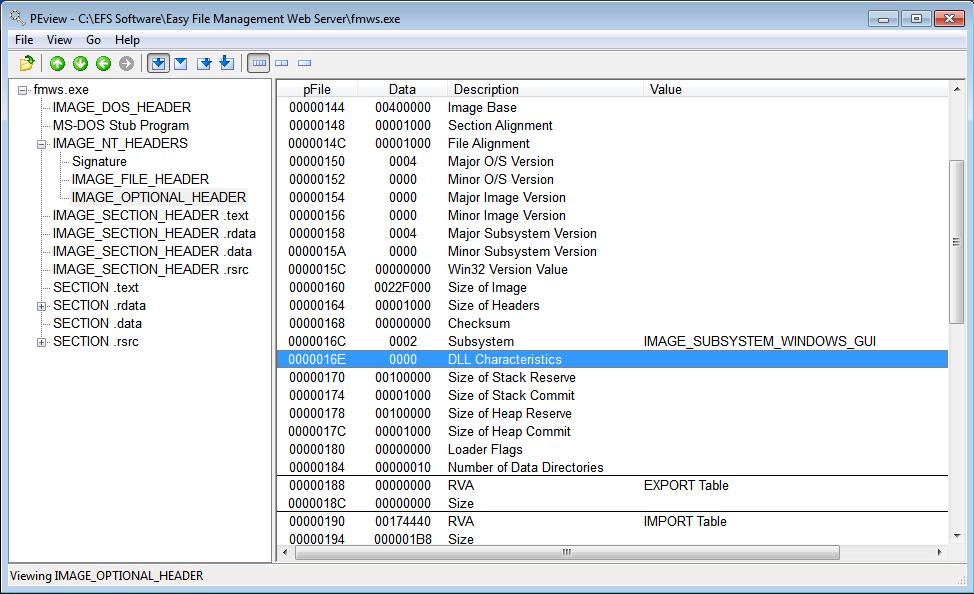
\includegraphics[width=\textwidth]{noASLRforfmws.png}
\end{figure}

From this can be seen that ImageLoad.dll is relocatable but ASLR is not enabled, and that fmws.exe is not relocatable and ASLR is not enabled.

%Now, with a hypothesis about our experiment from above (i. e. memory location for fmws.exe contra Imageload.dll and stack addresses will not change between debugging sessions or VM restarts), let us register relevant values and see if we can reject our hypothesis or not.

%We set a breakpoint at \texttt{kungfu} gadget's address (\escape{0x10022aac}) and also check when fmws.exe is entered and c.

%\begin{center}
  %\begin{tabular}{ | l | c | c | c }
    %\hline
   %- & \#1 & \#2 (debug sess) & \#3 (system reboot) \\ \hline
   % Memory address start IL &  0x00577000 & 0x00577000  & 0x00577000 \\ \hline
   % Stack address IL & 0x03E599FC & 0x03D399FC & 0x03FF99FC   \\ \hline
   % Memory address fmws &  0x77CB014D & 0x77CB014D & 0x750678D7   \\ \hline
   % Stack address fmws & 0x03B0FDF4 & 0x0393FDF4 & 0x001820D8   \\ \hline
  %\end{tabular}
%\end{center}

%(Sidenote: if breakpoint at 0x00457452, this is inside 0x00457451, which has value E8 FFE40C00 | CALL fmws.00525955. But, .52 has value ? FFE4 | JMP ESP .
%Guess this is the alignment exploit thingie.)

    \subsection{Assignment 5}

      The exploit uses the unprotected pats of the memory in the following way:

      \begin{verbatim}
   [ Explain how the exploit uses the
   unprotected memory to do the remote execution ]
      \end{verbatim}

    \subsection{Assignment 6}
One way to check if DEP is enabled for a program in Windows 8 is to open the Task Manager, go to the 'Processes' tab, open 'View' \escape{>} 'Select Columns...' and make sure the 'Data Execution Prevention' check button is checked. Press 'OK'. This then shows in the table if DEP is enabled for the different processes. When doing this on the virtual machine we could see that DEP was disabled for fmws.exe (see figure \ref{DEP}).

 \begin{figure}
	\caption{Screenshot of task manager with column DEP enabled, showing that DEP is disabled for fmws.exe.}\vspace{0.2em}
	\label{DEP}
	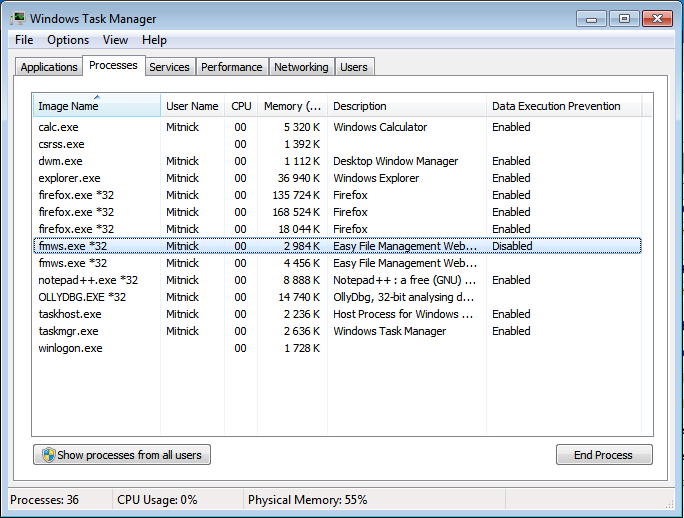
\includegraphics[width=\textwidth]{DEPdisabled-fmws.png}
\end{figure}


    \subsection{Assignment 7}

      The exploit could be modified in the following way to work under DEP:

      \begin{verbatim}
   [ Text explaining how the exploit could
     be modifed to work under DEP. ]
      \end{verbatim}

\end{document}
